\documentclass[11pt,a4paper]{article}

\usepackage{siunitx}
%\usepackage[version=4]{mhchem}
\usepackage{multirow}
\usepackage{subfig}

\usepackage{pgfgantt}
%\usepackage{pdflscape}
% \usepackage[a4paper,margin=1in,landscape]{geometry}

% \usepackage[pdftex]{color,graphicx}
% \pagestyle{plain}
\usepackage{geometry}
\usepackage{rotating}
\usepackage{hyperref}

\newcommand{\ts}{\textsuperscript}
\newcommand{\ic}{\texttt}
\newcommand\todo[1]{\textbf{TODO: #1}}

\sisetup{detect-weight=true, detect-family=true}

\usepackage[backend=biber,style=authoryear,sorting=nyt,dashed=false]{biblatex}
\renewcommand*{\nameyeardelim}{\addcomma\space}
\addbibresource{references/references.bib} % note the .bib is required

%Wrong spellings!
%parameterization (unless part of someone else's work)
%parameterizing
%Paracon

\begin{document}

% \newgeometry{margin=2.0cm}
\newgeometry{margin=2.2cm, top=2.5cm}

\begin{center}
    \Large{\textbf{Monitoring Committee Report V}}\\[0.1cm]
    \large{Mark Muetzelfeldt}\\
    \normalsize{11am on Thursday 14\ts{th} December 2017 in 2U13}\\[0.1cm]		
    \rule{\textwidth}{0.2mm}
    \textbf{Project Title: }Development of scale-awareness in the representation of
    convective cloud systems\\
    \textbf{Monitoring Committee: }Dr Omduth Coceal and  Dr Andrew Turner\\
    \textbf{Supervisors: }Prof. Robert Plant, Prof. Peter Clark, Dr Steve Woolnough \\
    and Dr Alison Stirling (Met Office CASE supervisor)\\
    \rule{\textwidth}{0.2mm}
\end{center}

\section{Project overview}
\label{sec:Project Overview}
% Overall goal.
% * represent the org of convection in a conv p13n
% * do in a scale-aware way.
% Steps to do this (see thesis structure notes)
% Stress physically justifiable
% Point out links between hi-res <=> p'trized
 

\subsection{Background reading}
\label{sec:Background reading}
% Conv p13n + org.
% Mapes and Neale 2011
% Willet and Whitall 2017
% Tompkins and Semie 2017
% Shear climatology
% Aiyyer and Thorncroft 2006
% Houchi et al. 2010
% Bonus
% Davies et al. 2009

\begin{itemize}
  \item \cite{mapes2011parameterizing}
  \item \cite{tompkins2017organization}
  \item \cite{willett2017simple}
  \item \cite{houchi2010comparison}
  \item \cite{aiyyer2006climatology}
  \item \cite{davies2009simple}
\end{itemize}

\section{Completed work}
\label{sec:Completed work}

\subsection{Progress overview}
\label{sec:Progress overview}

\subsection{Cloud tracking}
\label{sec:Cloud tracking}

\begin{figure}[htp!]%
    \centering
    \subfloat[label 1]{{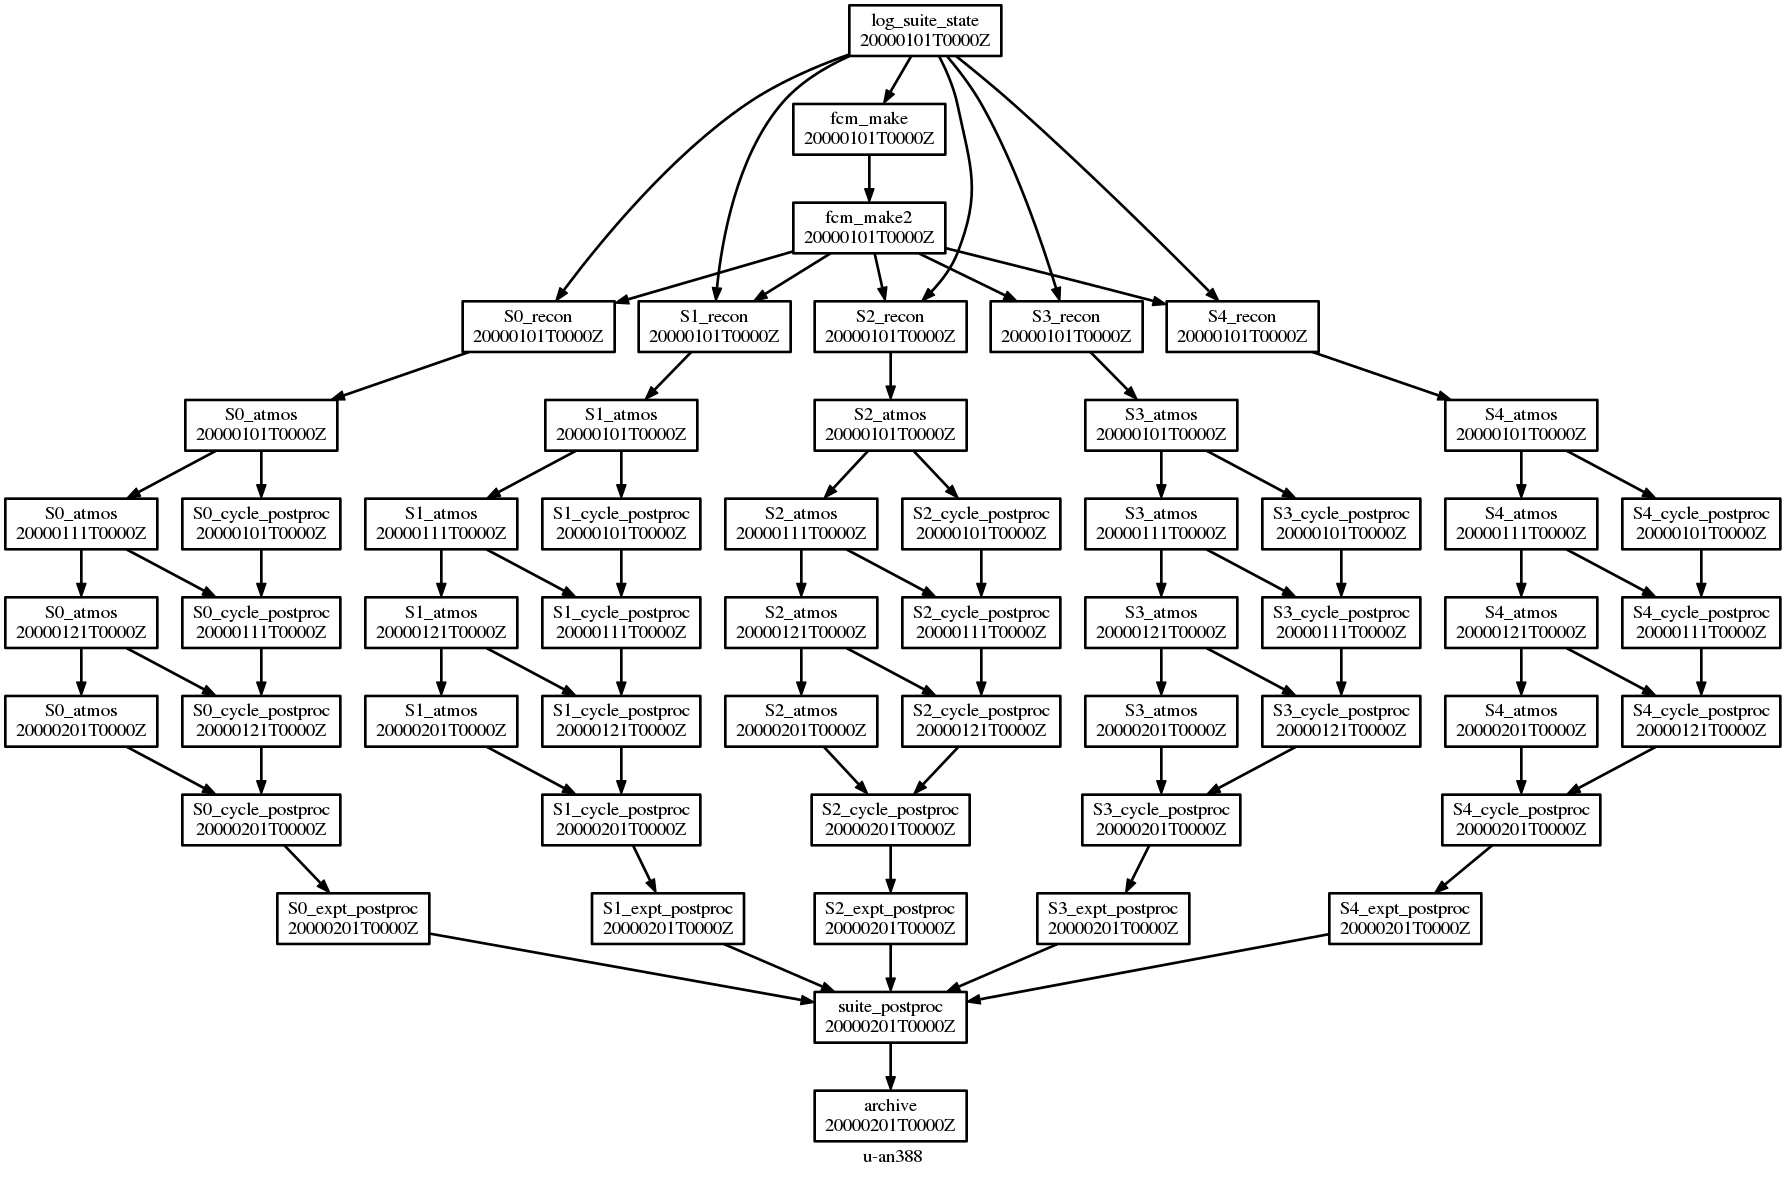
\includegraphics[width=5cm]{figs/u-an388_graph.png} }}%
    \qquad
    \subfloat[label 2]{{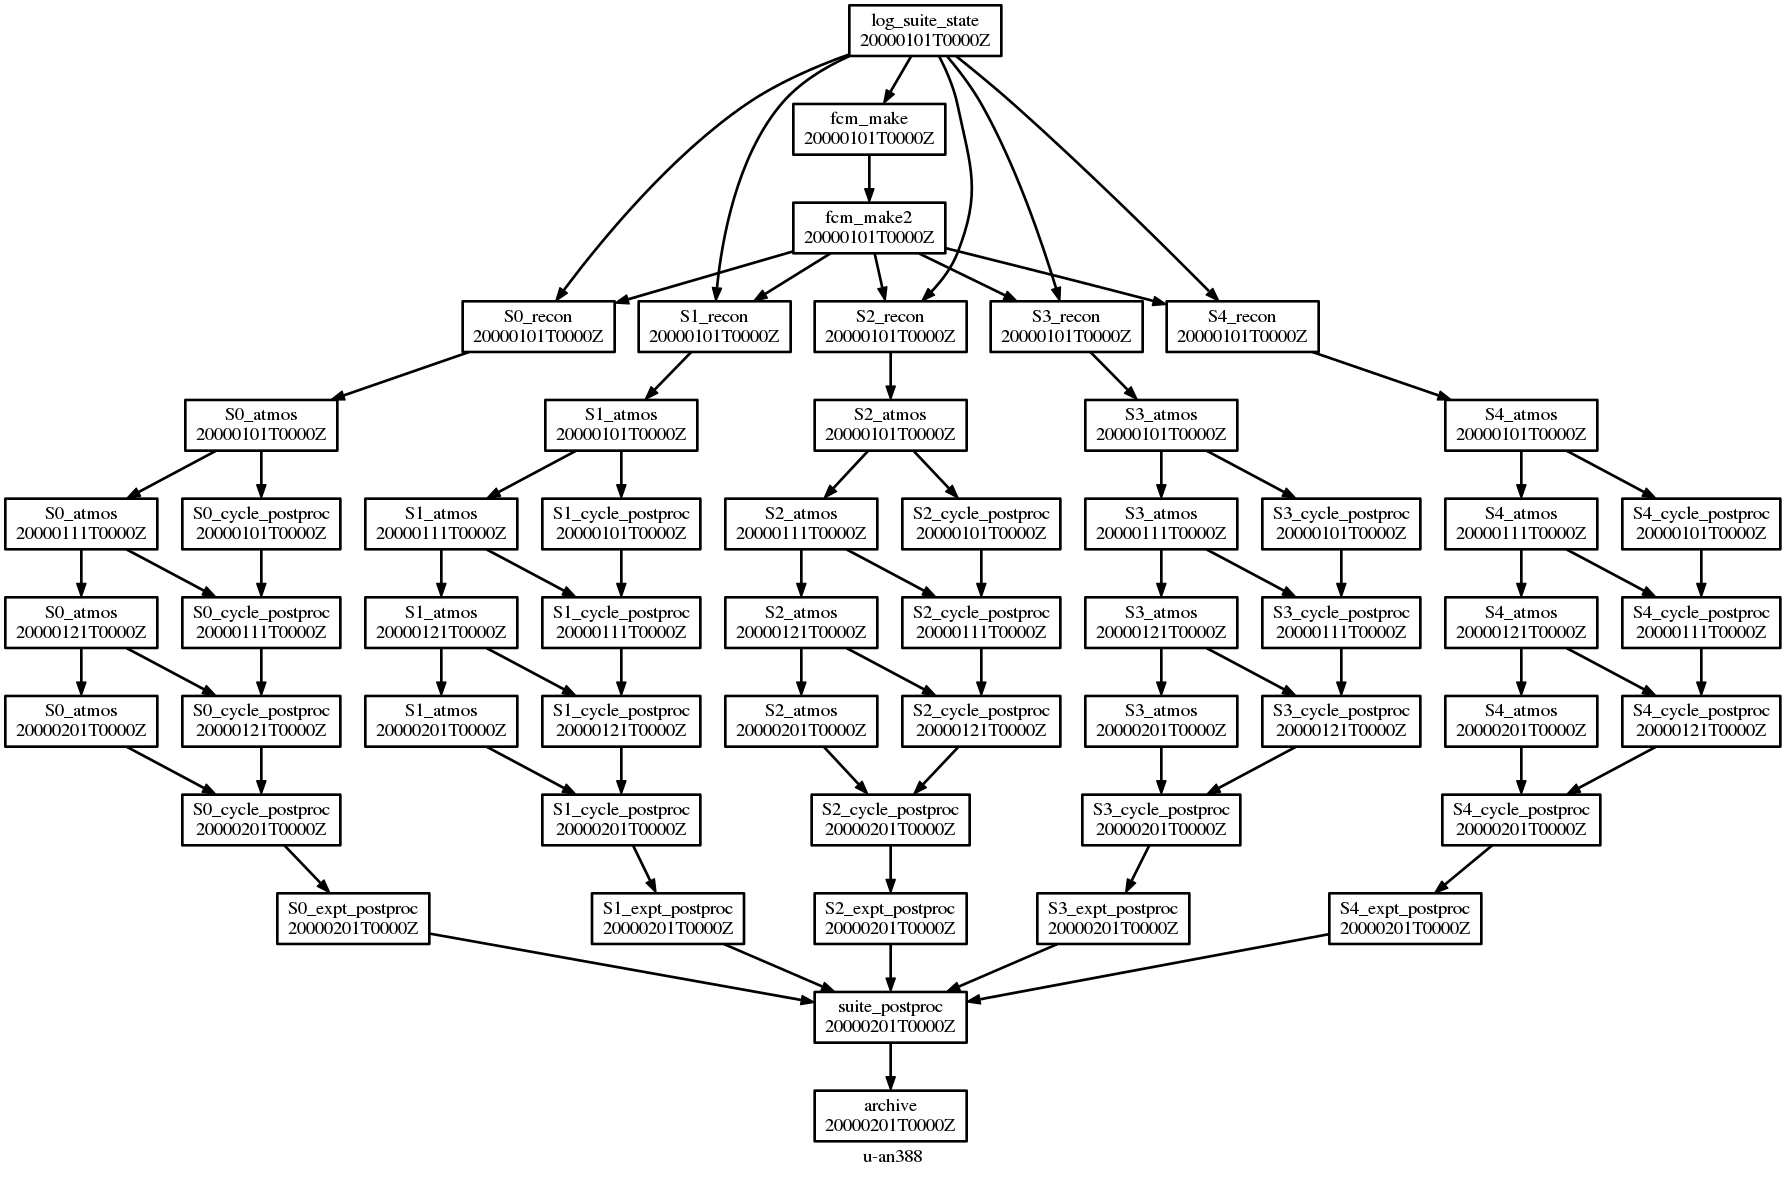
\includegraphics[width=5cm]{figs/u-an388_graph.png} }}%
    \caption{2 Figures side by side}%
    \label{fig:example}%
\end{figure}

\cite{wilson1998nowcasting},  \cite{plant2009statistical}

\subsection{Classification of shear profiles}
\label{sec:Classification of shear profiles}

\subsection{Modifications to the Met Office UM based on shear}
\label{sec:um_mod}

\section{Future work}
\label{sec:Future work}

\subsection{Shear climatology in the Met Office UM}
\label{sec:Shear climatology in the Met Office UM}

\subsection{High-resolution idealized modelling}
\label{sec:High-resolution idealized modelling}

\subsection{Writing 1}
\label{sec:Writing 1}

\section{Training record}
\label{sec:Training record}
% CMSS
% RRDPs

\subsection{Met Office placement}
\label{sec:Met Office placement}

\subsection{Posters, presentations and conferences}
\label{sec:presentations}
% Cambridge plenary
% Delft

\subsection{Transferable skills}
\label{sec:Transferable skills}
% PGR forum co-chair + org of QV.

\printbibliography[title={References}]

\newpage
\section*{Appendix}

\subsection*{PhD Timetable}

\begin{ganttchart}[vgrid, hgrid, y unit chart=0.75cm, MC/.style={milestone/.append style={shape=circle}}]{1}{20}  % <---
    \gantttitle{2017}{2}
    \gantttitle{2018}{12}
    \gantttitle{2019}{6} \\
    \gantttitle{N}{1}
    \gantttitle{D}{1}
    \gantttitle{J}{1}
    \gantttitle{F}{1}
    \gantttitle{M}{1}
    \gantttitle{A}{1}
    \gantttitle{M}{1}
    \gantttitle{J}{1}
    \gantttitle{J}{1}
    \gantttitle{A}{1}
    \gantttitle{S}{1}
    \gantttitle{O}{1}
    \gantttitle{N}{1}
    \gantttitle{D}{1}
    \gantttitle{J}{1}
    \gantttitle{F}{1}
    \gantttitle{M}{1}
    \gantttitle{A}{1}
    \gantttitle{M}{1}
    \gantttitle{J}{1} \\
    \ganttmilestone[MC, milestone left shift=0.2,milestone right shift=-0.2]{Monitoring committees}{2} 
    \ganttmilestone[MC, milestone left shift=0.2,milestone right shift=-0.2]{}{8} 
    \ganttmilestone[MC, milestone left shift=0.2,milestone right shift=-0.2]{}{14}  \\
    \ganttbar{Shear climatology}{2}{3} \\
    \ganttbar{High-resolution modelling}{3}{5} 
    \ganttmilestone{}{5} \\
    \ganttbar{Writing 1}{6}{8} 
    \ganttmilestone{}{8} \\
    \ganttbar{Idealized parametrized}{9}{11} \\
    \ganttbar{Global parametrized}{11}{13} 
    \ganttmilestone{}{13} \\
    \ganttbar{Writing 2}{13}{17} 
    \ganttmilestone{}{17} 
\end{ganttchart}

\subsection*{Repositories}

\begin{itemize}
  \item managing UM output: \href{https://github.com/markmuetz/omnium}{omnium}
  \item high-resolution analysis: \href{https://github.com/markmuetz/scaffold_analysis}{scaffold\_analysis}
  \item climatology of shear analysis: \href{https://github.com/markmuetz/cosar_analysis}{cosar\_analysis}
\end{itemize}

% Around 400 words.
\subsection*{Training record}
\subsubsection*{Year 1}

\begin{itemize}
  \item RRDP: Intermediate/Advanced \LaTeX\ (4/11/2015)
  \item RRDP: You and your supervisor (11/11/2015)
  \item RRDP: Quality assurance in research (18/11/2015)
  \item RRDP (equivalent): UM Training (16-18/12/2015)
  \item RRDP (equivalent): Preparing to teach: Introduction to teaching and learning (26/1/2016)
  \item Preparing to teach: Marking and feedback (26/1/2016)
  \item Preparing to teach: Laboratory demonstrating and leading small groups (27/1/2016)
  \item MONC Training course (9-10/2/2016)
  \item RRDP (equivalent): Fairbrother Lecture ``A slippery situation: melting ice in Antarctica'' (4/5/2016)
  \item ECMWF Parametrization of subgrid physical processes (16-20/5/2016)
\end{itemize}

\subsubsection*{Year 2}

\begin{itemize}
  \item RRDP: Managing your research project (17/11/2016)
  \item RRDP: How to write a thesis (24/1/2017)
  \item SCENARIO Data Assimilation Course (14-15/2/2017)
  \item RRDP: Presentation skills (7/3/2017)
  \item Software Development for scientists (8/3/2017, 28-29/3/2017)
\end{itemize}

\subsubsection*{Year 3}

\begin{itemize}
  \item NCAS Climate Modelling Summer School: demonstrating Numerical Methods for Hilary Weller (11-15/11/2017)
  \item CASE Met Office Placement (30/10/2017 - 24/11/2017)
  \item RRDP: Open access for research publications (27/11/2017)
  \item RRDP: Introduction to impact (30/11/2017)
\end{itemize}

\subsection*{Talks and conferences attended}

\begin{itemize}
  \item Climate Change 2013: The physical science basis. Institute of Physics (2/2014)
  \item Dame Julia Slingo: Taking the planet into uncharted territory: What climate models can tell us about the future (9/2014)
  \item SCENARIO NERC DTP Conference (9/6/2015)
  \item Climate Change in the run-up to the Paris conference: what has Physics got to say? (6/11/2015)
  \item RMetS talk: The risk and vulnerability of Europe to severe convective storms (6/4/2016)
  \item ParaCon Plenary 1 in Reading (27-28/6/2016)
  \item RMetS debate: What will make the public and politicians take climate change more seriously? (5/10/2016)
  \item RMetS talks: Come Rain or Come Shine (19/10/2016)
  \item COP22 Marrakech: Remote participation (11/11/2016)
  \item ParaCon plenary 2 in Leeds (6-7/12/2016)
  \item RMetS talks: Chaos and Confidence in Weather Forecasting (14/12/2016)
  \item ParaCon plenary 3 in Cambridge (3-4/7/2017)
  \item The Future of Cumulus Parametrization, Delft University of Technology (10-14/7/2017)
  \item ParaCon plenary 4 in Exeter (18-19/12/2017)
  \item (Planned) EGU: Vienna (8-13/4/2018)
\end{itemize}

\subsection*{Talks and conferences presented at}

\begin{itemize}
  \item Presentation: ``Effects of Shear on Cloud Field Organization''. \textit{Quo Vadis}, University of Reading (1/2/2017)
  \item Poster: ``Effects of Shear on Cloud Field Organization''. Met Office Academic Partnership (MOAP), Met Office, Exeter (22/2/2017)
  \item Poster: ``Effects of Vertical Shear on Cloud Field Organization and Variability''. The Future of Cumulus Parametrization, Delft University of Technology (10-14/7/2017)
  \item Poster: ``Effects of Vertical Shear on Cloud Field Organization and Variability''. PhD Poster Session (21/9/2017)
\end{itemize}

\end{document}
